\chapter{Development Analysis}
\section{Literature Review}
Research post component selection was completed largely using the provided \gls{ti} documentation for the specific device.
\subsection{Intelligent Stepper Motor Driver with DRV8811/18/24/25}
This document is provided as a supplement to the DRV8811/18/21/24/25 data sheets. 
It provided an analogous solution for comparison to the algorithms developed on C2000 platform.
It details a technique to improve real time control of an internal indexer bipolar stepper motor driver such as the DRV8825 while obtaining programmable acceleration and deceleration profiles, speed control and position control by the utilization of a conventional MSP430 microcontroller and any of the aforementioned power stages.\cite{dev_intelligent}

\subsection{Programming TMS320x28xx and 28xxx Peripherals in C/C++}
This application report explores a hardware abstraction layer implementation to make C/C++ coding easier on C28x devices. 
This method is compared to traditional \#define macros and topics of code efficiency and special case registers are also addressed.\cite{dev_peripherals}
It was used to solve issues related to the analog GPIO systems present on the C2000, and increase over all system efficiency.

\subsection{TMS320C28x Optimizing C/C++ Compiler v6.2.4}
This user's guide discusses the characteristics of the C/C++ compiler.
It provides an overview of these tools and introduces the features of the optimizing C/C++ compiler. 
The assembler and linker are also discussed in detail.\cite{dev_optimize}
It was used for researching new compiler optimizations referenced in the Programming TMS320x28xx and 28xxx Peripherals in C/C++ documentation.

%other people can post their docs.

\section{Concept Generation}
Figure ~\ref{fig:architecture} shows the overall architecture of the Senior Thesis Project, which is fully specified by Table ~\ref{table:zerolevel}.

\begin{figure}[h]
	\centering
	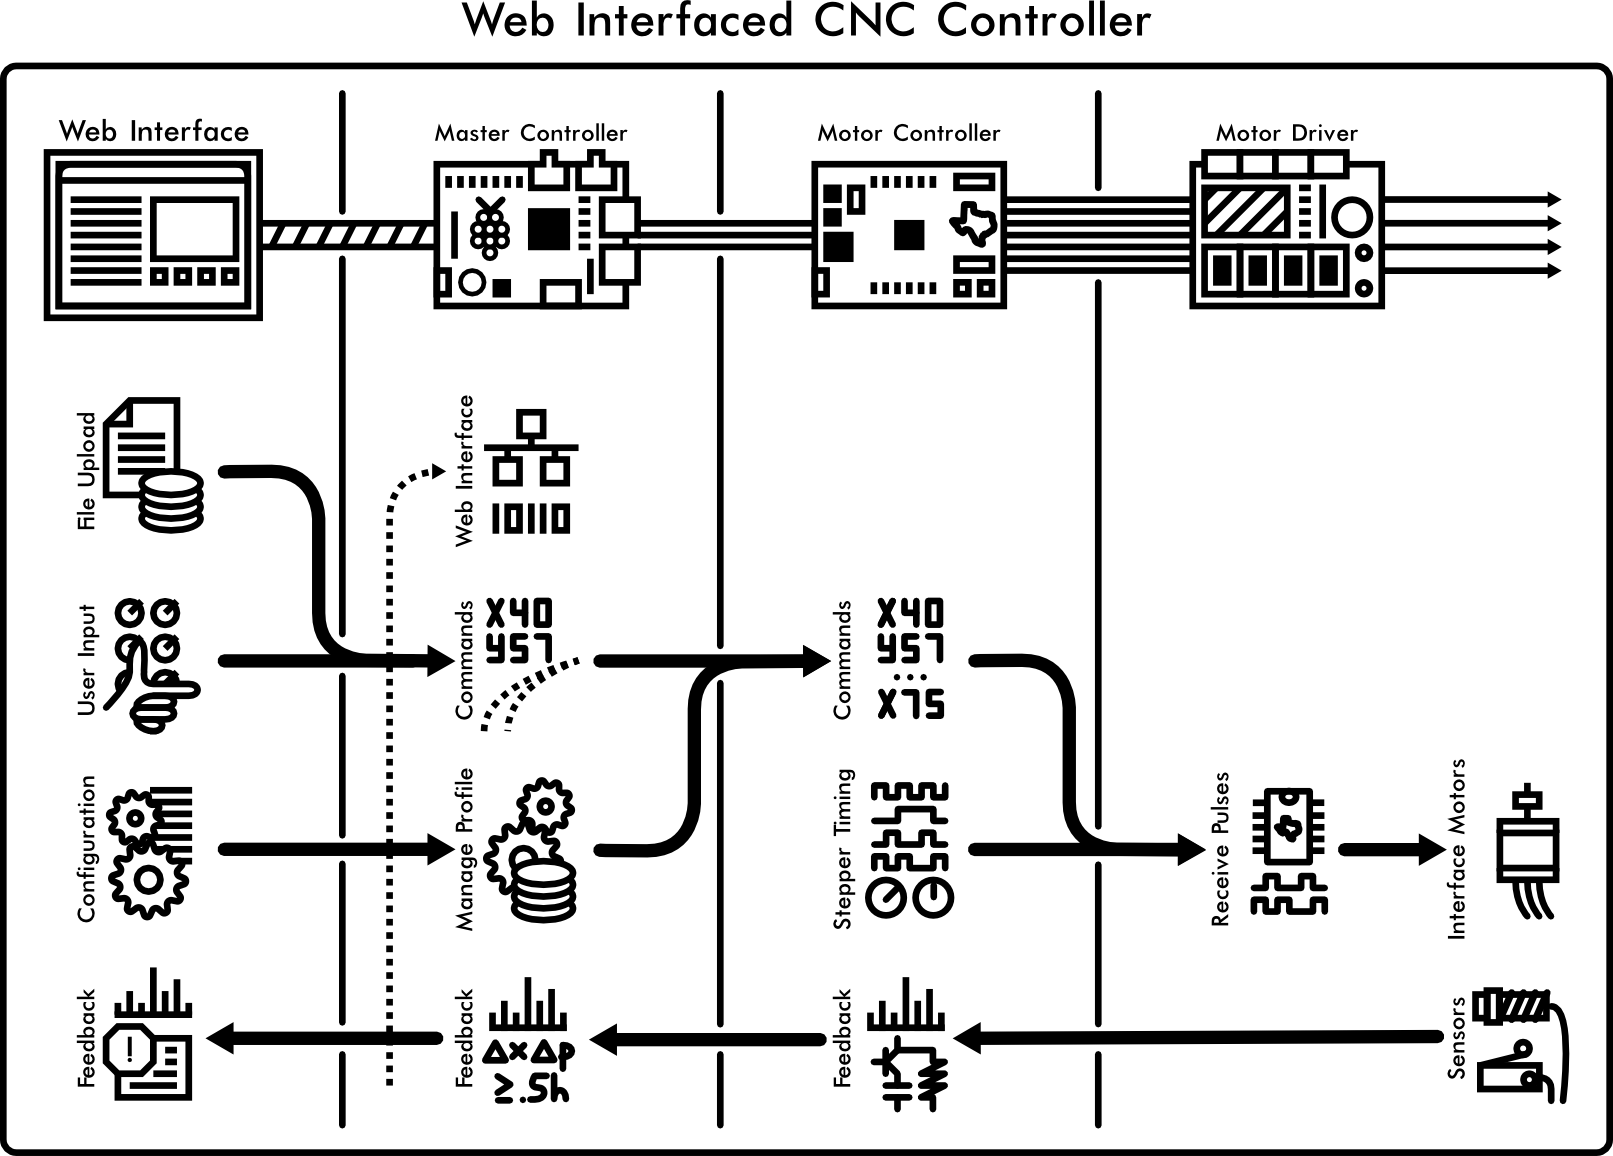
\includegraphics[width=1\textwidth]{architecture.png}
	\caption{System Architecture}
	\label{fig:architecture}
\end{figure}

\section{Concept Reduction}
%\section{Production Schedule}